\documentclass[12pt, a4paper, portrait]{article}
%Gummi|065|=)
\usepackage[affil-it]{authblk}
\usepackage{hyperref}
\hypersetup{
  colorlinks=true,
  linkcolor=black,
  filecolor=magenta,
  urlcolor=blue
}
\urlstyle{same}
\usepackage{indentfirst}
\usepackage{courier}
\usepackage{listings}
\usepackage{color}
\definecolor{codegreen}{rgb}{0,0.6,0}
\definecolor{codegray}{rgb}{0.5,0.5,0.5}
\definecolor{codepurple}{rgb}{0.58,0,0.82}
\definecolor{backcolour}{rgb}{0.95,0.95,0.92}
\lstdefinestyle{mystyle}{
    backgroundcolor=\color{backcolour},   
    commentstyle=\color{codegreen},
    keywordstyle=\color{magenta},
    numberstyle=\tiny\color{codegray},
    stringstyle=\color{codepurple},
    basicstyle=\ttfamily\footnotesize,
    breakatwhitespace=false,         
    breaklines=true,                 
    captionpos=b,                    
    keepspaces=true,                 
    numbers=left,                    
    numbersep=5pt,                  
    showspaces=false,                
    showstringspaces=false,
    showtabs=false,                  
    tabsize=2
}
 
\lstset{style=mystyle}

\usepackage{indentfirst}
\usepackage[utf8]{inputenc}

\usepackage{titlesec}
\setcounter{secnumdepth}{4}
\setcounter{tocdepth}{4}

\titleformat{\paragraph}
{\normalfont\normalsize\bfseries}{\theparagraph}{1em}{}
\titlespacing*{\paragraph}
{0pt}{3.25ex plus 1ex minus .2ex}{1.5ex plus .2ex}

\usepackage{geometry}
\geometry{
 a4paper,
 left=20mm,
 top=20mm,
 right=25mm,
 bottom=20mm
}

% Personal data
\title{\textbf{Sensor Music Player}}
\author{István Szőllősi}
\affil{Faculty of Sciences and Letters, ``Petru Maior'' University of Târgu Mureș}
\date{August 25, 2018}

\renewcommand{\baselinestretch}{1.5} 
\usepackage{graphicx}

\begin{document}

\maketitle
\newpage

\tableofcontents
\newpage

\section{About}
I would like to present how to gain values from an accelerometer and process that data on a separate server.\newline The scopes of the project:
\begin{itemize}
\item{main scope - make a music player that can be controlled with gestures}
\item{understable and optimized signal processing (FastDTW, Dtaidistance, etc)}
\item{easily buildable/usable server side (Node.js, Express.js, PythonShell)}
\end{itemize}
\par Listen to music can be a relaxing activity or source of motivation for some people. Many people always listen to music when he/she has possibility.
Nowadays almost everybody use a smart device to listen to music.
People listen to music in there cars, in there homes, in the office, on the bus/train almost in every places.
\par To control the music player you need to touch the device at least once a time if you are in the car or if the screen of a smart device is open.
But, if your music player device is in your pocket, you at first need to pull out, to unlock the screen, to open the music player app and for the last time to change your track.
This is a long way to change a track and in some case it is hard to execute for example on a bus/train with many people.
\par To resolve these problems we can use a music player which can be controlled with gestures. From this time we do not need to unlock everytime a smart device to change a track or we do not need to pull out from our pocket.
We can easily change a track if the device is in our pocket by double tap the topside of the device.
\par The player monitors the state changes of the accelerometer and with a help of a server can analyze in almost real-time what type of gesture is and what to do.
\subsection{Technical about}
\par The main structure of the repository is
\textit{a valid Android project} with several additionals folders, like the:
\begin{itemize}
\item{\textbf{backend}} folder where the \textit{Python} and \textit{JavaScript} code is stored
\item{\textbf{docs}} folder where the documents about the project are stored
\end{itemize}
\par Source code available: \url{https://github.com/I-sty/SensorMusicPlayer/}.
\subsection{Workflow}
\begin{enumerate}
\item{Use the Android application to get the values from the accelerometer}
\begin{enumerate}
\item{Navigate to \textit{Config activity}}
\item{Press the \textit{Record} button to start recording the accelerometer}
\begin{itemize}
\item{The text of the button will be changed to \textit{Stop}}
\end{itemize}
\item{Press the \textit{Stop} button to stop recording}
\item{Press the \textit{Send} button to send the recorded signal to the Node.js server}
\item{Optionally, you can "analyze" your recorded array by pressing the \textit{Analyze} button}
\begin{itemize}
\item{This feature checks your items in the array if they are greater than a predefined threshold.}
\item{This feature eliminates the ability to send almost blank lists to the server}
\end{itemize}
\end{enumerate}
\item{By pressing the \textit{Send} button in Android application, the application sends the recorded list to the server using a REST POST call.}
\item{The Node.js server receives the request from the application and process it.}
\begin{enumerate}
\item{\textbf{REST API level} - The request arrives to the right URI path, that was registrated to receive request.}
\item{\textbf{Controller level} - The \textit{REST API level} forwards the request to the right function of the controller.}
\begin{enumerate}
\item{The body of the request is forwarded to the \textit{Model level} to parse. The return object will be saved in MongoDB.}
\item{The body of the request is forwarded to another function where the DTW's distance will be calculated using the PythonShell module.}
\end{enumerate}
\item{\textbf{Model level} - The body of the request will be interpreted as a \textit{Mongoose} object and returned to the \textit{Controller level} so it can be saved.}
\end{enumerate}
\item{The calculated distance will be send to the Android application as a respond for the POST request.}
\end{enumerate}


\pagebreak
\section{Node.js}
In Node.js is very simple to create a small web server for REST calls.
\subsection{Installation}
\begin{lstlisting}[language=bash]
sudo apt install nodejs
\end{lstlisting}
\subsection{Usage}
To start use the follow command in the project's folder:
\begin{lstlisting}[language=bash]
npm run start
\end{lstlisting}
\subsection{Configuration}
Used tutorial: \href{https://www.codementor.io/olatundegaruba/nodejs-restful-apis-in-10-minutes-q0sgsfhbd}{Build Node.js RESTful APIs in 10 Minutes}
\subsubsection{Mongoose}
Mongoose is an Object Data Modeling (ODM) library for MongoDB and Node.js. It manages relationships between data, provides schema validation, and is used to translate between objects in code and the representation of those objects in MongoDB.
\paragraph{Installation}
\begin{lstlisting}[language=bash]
npm install mongoose
\end{lstlisting}
\subsubsection{Express}
Express.js, or simply Express, is a web application framework for Node.js. It is designed for building web applications and APIs
\paragraph{Installation}
\begin{lstlisting}[language=bash]
npm install express --save
\end{lstlisting}
\subsubsection{Nodemon}
\textit{nodemon} is a tool that helps develop node.js based applications by automatically restarting the node application when file changes in the directory are detected.
\paragraph{Installation}
\begin{lstlisting}[language=bash]
npm install --save-dev nodemon
\end{lstlisting}

\pagebreak
\section{MongoDB}
MongoDB to store signal data from the \textit{Y axis} of the accelerometer from the Android devices.
\subsection{Installation}
\begin{lstlisting}[language=bash]
sudo apt install mongodb
\end{lstlisting}
\subsection{Runing}
To start mongo service use the follow command:
\begin{lstlisting}[language=bash]
sudo mongod --config /etc/mongodb.conf 
\end{lstlisting}
\subsection{Drop a collection}
In some cases you need to drop collections, for example when the collections contains random test cases what were introduced during the development process.
\par To drop/clear a collection introduce the following codes, in the Mongo's shell.
\par To access the Mongo's shell enter the \textit{mongod} command in terminal.
\begin{lstlisting}[language=bash, caption=MongoDB shell commands to drop a collection]
show dbs
use <db>
show collections
db.<collection>.drop()
\end{lstlisting}

\pagebreak
\section{Matplotlib}
Matplotlib is a plotting library for the Python programming language.
I used \textit{matplotlib} to generate graphical view of my series.
\subsection{Installation}
Install module using this \href{https://matplotlib.org/users/installing.html#linux-using-your-package-manager}{tutorial}.
\par Optionally, you need to install the \textbf{python-tk} package also.
\subsection{Examples}
According to this \href{https://matplotlib.org/users/pyplot_tutorial.html}{official tutorial} you can easily generate a plot about an array using this Python script:
\begin{lstlisting}[language=Python]
import matplotlib.pyplot as plt
plt.plot([ 5.733, 1.704, -2.713, -1.343, 2.604, 3.922, 2.157, -0.910, -2.414, -2.943, -1.526, -0.823])
plt.ylabel('some numbers')
plt.show()
\end{lstlisting}

Result:
\begin{figure}[ht]
\centering
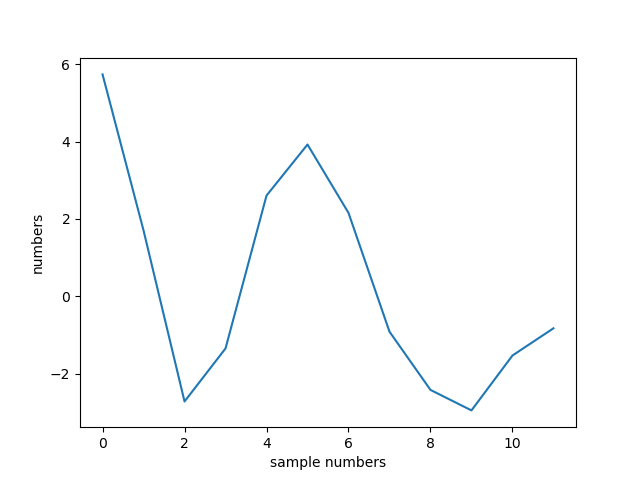
\includegraphics[scale=0.83]{Figure_2.png}
\caption{The result of the script}
\end{figure}
\clearpage
This example was very easy, so here is a \textit{normal} signal from the accelerometer:
\begin{figure}[htp]
\centering
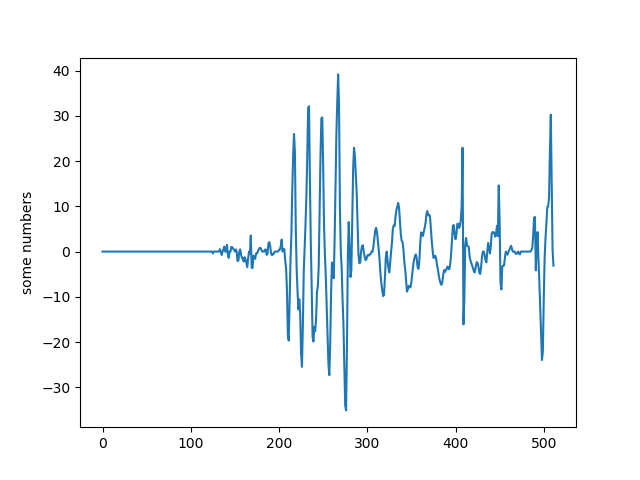
\includegraphics[scale=1.00]{Figure_1.png}
\caption{A section of the signal of accelerometer in real usage}
\end{figure}

\pagebreak
\section{DTAIDistance}
Library for time series distances (e.g. Dynamic Time Warping) used in the \href{https://dtai.cs.kuleuven.be/}{DTAI Research Group}.
\par
DTAIDistance official documentation: \href{https://dtaidistance.readthedocs.io/en/latest/index.html}{dtaidistance.readthedocs.io}
\par Source available on \url{https://github.com/wannesm/dtaidistance}.

\subsection{Installation}
Run the follow codes in terminal to install the module:
\begin{lstlisting}[language=bash, caption=Used Linux Mint 19]
sudo apt install python3-pip python3-setuptools  python3-dev python3-tk
pip3 install wheel
pip3 install dtw
pip3 install dtaidistance
\end{lstlisting}

\subsection{Usage}
\begin{lstlisting}[language=Python, caption=Script to calculate DTW distance and plot warping paths matrix ]
from dtaidistance import dtw
from dtaidistance import dtw_visualisation as dtwvis
import numpy as np

s1 = np.array([0, 1, 2, 1, 0, 2, 1, 0, 0])
s2 = np.array([0, 1, 2, 1, 0, 0, 1, 2, 1])

d, matrix = dtw.warping_paths(s1, s2, window=25, psi=2)
print('DTW distance = ', d)

dtwvis.plot_warpingpaths(s1, s2, matrix, best_path, "image.png")
\end{lstlisting}

\clearpage
The result will be put in the newly created \textbf{image.png} file.
\begin{figure}[ht]
\centering
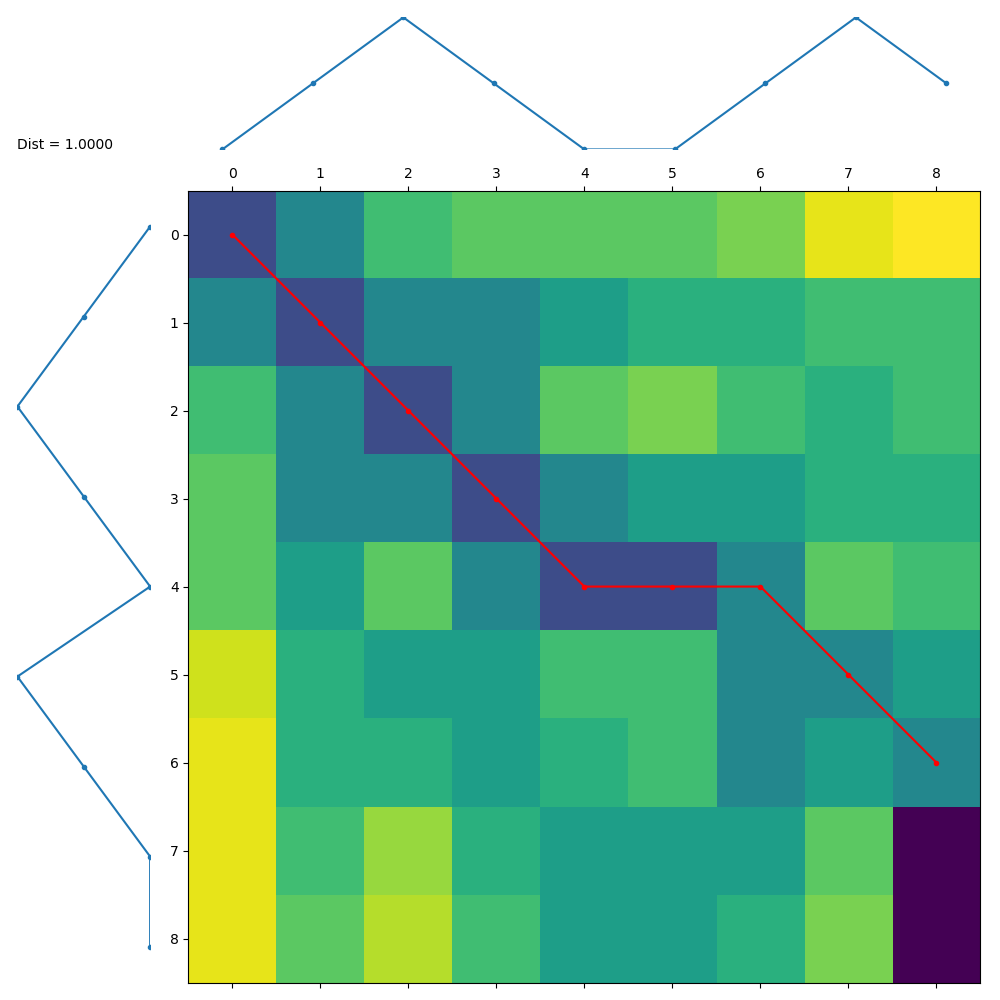
\includegraphics[scale=0.60]{dtaidistance-sample.png}
\caption{DTAIDistance's warping paths matrix}
\label{}
\end{figure}

\subsection{Documentation}
\begin{lstlisting}[language=Python]
import numpy as np
s1 = np.array([0, 1, 2, 1, 0, 2, 1, 0, 0])
\end{lstlisting}
\par\href{http://www.numpy.org/}{NumPy} is a library for the Python programming language, adding support for large, multi-dimensional arrays and matrices, along with a large collection of high-level mathematical functions to operate on these arrays.
\par The \textit{array()} function creates an array from a given list. See more details \href{https://docs.scipy.org/doc/numpy/reference/generated/numpy.array.html#numpy.array}{here}.
\newline
\begin{lstlisting}[language=Python]
from dtaidistance import dtw
d, matrix = dtw.warping_paths(s1, s2, window=25, psi=2)
print('DTW distance = ', d)
print('DTW matrix = ', matrix
\end{lstlisting}

\par The \textit{warping\_paths()} function calculates the DTW distance and the DTW matrix for the two given series. See more details
\href{https://dtaidistance.readthedocs.io/en/latest/modules/dtw.html?highlight=warping_paths#dtaidistance.dtw.warping_paths}{here}.
\newline

\begin{lstlisting}[language=Python]
from dtaidistance import dtw_visualisation as dtwvis
dtwvis.plot_warpingpaths(s1, s2, matrix, best_path, "image.png")
\end{lstlisting}
\par The \textit{plot\_warpingpaths()} method plots the warping paths matrix into the \textit{image.png} file. See more details \href{https://dtaidistance.readthedocs.io/en/latest/modules/dtw_visualisation.html}{here}.


\pagebreak
\section{Postman}
\subsection{Installation}
Installed according to this article: \href{https://r00t4bl3.com/post/how-to-install-postman-native-app-in-linux-mint-18-3-sylvia}{How to install Postman native app in Linux Mint 18.3}

Used to test the main functionalities of the Node.js server.

\subsection{Usage}
\subsubsection{GET}
To get all buffers from database run this code in Postman/Linux terminal
\begin{lstlisting}[language=bash, caption=Get all buffers]
curl -X GET http://localhost:3000/buffers
\end{lstlisting}

The response is or an empty list, if no items in the database or a list like this:
\begin{lstlisting}[language=XML, caption=A sub section of the signal to process]
[
    {
        "value": [
            5.733050346374512,
            1.704751968383789,
            -2.7134790420532227,
            -1.343064308166504,
            2.6042985916137695,
            3.92281436920166,
            2.15725040435791,
            -0.9106369018554688,
            -2.4146032333374023,
            -2.943338394165039,
            -1.5269522666931152,
            -0.8230304718017578
        ],
        "_id": "5b82607f5601ec575d3bf0e4",
        "__v": 0
    }
]
\end{lstlisting}

\subsubsection{POST}
Post a new buffer a.k.a a sub section of the signal to store and process. Run this code in Postman or in a Linux terminal to post a new buffer to the Node.js server.
\begin{lstlisting}[language=bash, caption=Send signal data via REST]
curl -X POST http://localhost:3000/buffers  -d '{
	"value":[-2.2, -1.1, 0, 1.1, 2.2]
}'
\end{lstlisting}

\pagebreak
\section{PyMongo}
Use \href{https://github.com/mongodb/mongo-python-driver}{PyMongo} if you want to get items from your MongoDB and want to parse in Python environment.
\subsection{Installation}
\begin{lstlisting}[language=bash]
pip3 install pymongo
\end{lstlisting}
Installing with pip: \url{http://api.mongodb.com/python/current/installation.html}
\subsection{Usage}
\begin{lstlisting}[language=Python]
import pymongo
from pymongo import MongoClient
client = MongoClient('localhost', 27017)
client.database_names()
db = client['<db_name>']
db.collection_names()
coll = db['<collection_name>']

for col in coll.find({}):
  for keys in col.keys(): 
    if keys == "value":
      print ('{', keys, ":" , col[keys] , '}' )
    print('\n')
        
\end{lstlisting}

\pagebreak
\section{PythonShell}
Use \href{https://github.com/extrabacon/python-shell}{PythonShell} if you want to call a Python script in Node.js environment. For example when you receive a POST request in the Node.js server and you want to process your data using a Python script.
\subsection{Installation}
\begin{lstlisting}[language=bash]
sudo npm install python-shell
\end{lstlisting}
\subsection{Usage}
\begin{lstlisting}[language=Python]
var PythonShell = require('python-shell');

function callPythonMethod(req, res){
  var options = {
    mode: 'text',
    pythonPath: 'python3', // or use the command
    pythonOptions: ['-u'], // get print results in real-time
    scriptPath: '<fullPathToTheFolder>/backend/python/',
    args: [req]
  };
  PythonShell.run('<script>.py', options, function (err, results) {
    if (err) res.send(err);
    res.json(results);
  });
};
\end{lstlisting}
\subsection{Integrate into the project}
You need to add these lines of code into the method where you create and save a new MongoDB item. The first step is to convert the input paramater a.k.a the body of the request to JSON object. From this JSON object you can get the array, convert to string and pass to the \textit{callPythonMethod()} as first parameter.
\begin{lstlisting}[language=Java]
exports.create_a_buffer = function(req, res) {
  var new_buffer = new Buffer(req.body);
  new_buffer.save(function(err, task) {
    if (err) res.send(err);
    //res.json(task);
  });
  
  var stringify = JSON.stringify(req.body);
  var body = JSON.parse(stringify);
  callPythonMethod(body.value.toString(), res);
};
\end{lstlisting}

\end{document}
